\documentclass[final]{beamer}
\usepackage[scale=1.24]{beamerposter}
\usetheme{confposter} % Use the confposter theme supplied with this template

\usepackage{multicol,lipsum}
\usepackage{graphicx}	% Required for including images
\usepackage{booktabs} % Top and bottom rules for tables	
\usepackage[fleqn,tbtags]{mathtools}	
\newtheorem{thm}{Theorem}
\newtheorem{defi}{Definition}
\newtheorem{prop}{Proposition}

\usepackage{amsfonts}
\usepackage[T1]{fontenc}
\usepackage{lmodern}

%-----------------------------------------------------------
% Define the column width and poster size
%
% To set effective sepwid, onecolwid and twocolwid values, first choose how many columns you want and how much separation you want between columns
% Then set onecolwid to be (1-(#cols+1)*separation))/#cols
% And set twocolwid to be 2*onecolwid + separation 
%
% In the template, the chosen number of columns is 4 and the separation is 0.024
% Thus, onecolwid = (1-(4+1)*0.024))/4= 0.22
% And twocolwid = 2*onecolwid + 0.024 = 0.464
%-----------------------------------------------------------

%-----------------------------------------------------------
% Define the column widths and overall poster size
% To set effective sepwid, onecolwid and twocolwid values, first choose how many columns you want and how much separation you want between columns
% In this template, the separation width chosen is 0.024 of the paper width and a 4-column layout
% onecolwid should therefore be (1-(# of columns+1)*sepwid)/# of columns e.g. (1-(4+1)*0.024)/4 = 0.22
% Set twocolwid to be (2*onecolwid)+sepwid = 0.464
% Set threecolwid to be (3*onecolwid)+2*sepwid = 0.708

\newlength{\sepwid}
\newlength{\onecolwid}
\newlength{\twocolwid}
\newlength{\threecolwid}
\setlength{\paperwidth}{48in} % A0 width: 46.8in
\setlength{\paperheight}{36in} % A0 height: 33.1in
\setlength{\sepwid}{0.001\paperwidth} % Separation width (white space) between columns
\setlength{\onecolwid}{0.22\paperwidth} % Width of one column
\setlength{\twocolwid}{0.464\paperwidth} % Width of two columns
\setlength{\threecolwid}{0.708\paperwidth} % Width of three columns
\setlength{\topmargin}{-0.5in} % Reduce the top margin size


%-----------------------------------------------------------
% Define colors (see beamerthemeconfposter.sty to change these colour definitions)
%-----------------------------------------------------------

\setbeamercolor{block title}{fg=ngreen,bg=white} % Colors of the block titles
\setbeamercolor{block body}{fg=black,bg=white} % Colors of the body of blocks
\setbeamercolor{block alerted title}{fg=white,bg=dblue!70} % Colors of the highlighted block titles
\setbeamercolor{block alerted body}{fg=black,bg=dblue!10} % Colors of the body of highlighted blocks
% Many more colors are available for use in beamerthemeconfposter.sty


%-----------------------------------------------------------
% Name and authors of poster/paper/research
%-----------------------------------------------------------

\title{The Hausdorff Dimension of Limit Sets of Well-distributed Schottky Groups} % Poster title
\author{William Huanshan Chuang} % Author(s)
\institute{Mathematics Department, San Francisco State University} % Institution(s)

%-----------------------------------------------------------
% Start the poster itself
%-----------------------------------------------------------
% The \rmfamily command is used frequently throughout the poster to force a serif font to be used for the body text
% Serif font is better for small text, sans-serif font is better for headers (for readability reasons)
%-----------------------------------------------------------

\begin{document}
\addtobeamertemplate{block end}{}{\vspace*{2ex}} % White space under blocks
\addtobeamertemplate{block alerted end}{}{\vspace*{2ex}} % White space under highlighted (alert) blocks

\setlength{\belowcaptionskip}{2ex} % White space under figures
\setlength\belowdisplayshortskip{2ex} % White space under equations
	
\begin{frame}[t] % The whole poster is enclosed in one beamer frame

\begin{columns}[t]% The whole poster consists of three major columns, the second of which is split into two columns twice - the [t] option aligns each column's content to the top

\begin{column}{\sepwid}\end{column}% empty spacer column


\begin{column}{\onecolwid} % The first column

%----------------------------------------------------------------------------------------
%	OBJECTIVES
%----------------------------------------------------------------------------------------

\begin{alertblock}{Abstract}
\begin{small}
Let a finitely generated Schottky group $G$ be given, and $\mathbb{B}^2$ be a Poincar\'{e} disk model of two-dimensional hyperbolic space. An unsolved problem is: How to find an exact value of Hausdorff dimension of the limit set $L(G)$ when $L(G)\neq \partial \mathbb{B}^2$? 

To solve one specific case of this problem, a well-distributed Schottky group $\Gamma=\left\langle T_1,T_2,...,T_m\right\rangle$ is defined. Our main theorem was proved based on: properties of Poincar\'{e} series, isometric circles, and some nice properties come with the definition of well-distributed Schottky group, especially that we found a way to reconstruct the orbit $\Gamma(0)$ by using only two operators $T$ and $R$ for any $m\in\mathbb{Z}^+$. 

\end{small}
\end{alertblock}

\begin{block}{Motivation}
\begin{small}
The following are five top historical reasons that highlight the need of creating a systematic method for computing the critical exponent of the Poincar\'{e} sereis. Let $G$ be a finitely generated Schottky group. 

\end{small}
\begin{small}
\begin{itemize}
\item In the prime geodesic theorem\cite{borthwick2007spectral}, $\delta(G)$ plays a role $z = \delta(G) + it$ which is similar to the line $z=1$ in the prime number theorem where the Riemann zeta function has its only singularity at the point $z = 1$ and no zeros on this line as proved by von Mangoldt in 1895.
\item In the spectral gap problem of hyperbolic surfaces\cite{bourgain2018spectral}, a hyperbolic surface has an essential spectral gap if it can meet some conditions in the theorem they proved, meaning that there are finitely many zeros within the region $\Re(s)>\frac{1}{2}-\beta=\delta(G)$.
\item In $\text{AdS}_3/\text{CFT}_2$\cite{dong2018phase}, $\delta(G)$ is a criterion for the critical exponent of a scalar field to have stable solutions in 3d quantum gravity. 
\item Since $\delta(G)$ uniquely determines the first resonance of the corresponding Selberg zeta function of $G$, and the first resonance is the lowest eigenvalue of eigenfunctions of the Laplacian operated on a Riemann surface (algebraic curve) $\mathbb{H}^2/G$. Since $\delta(G)$ is the convergence exponent of Poincar\'{e} series of $G$, and this series can be written into a Dirichlet $L-$function, plus eigenfunctions of $\mathbb{H}^2/G$ are automorphic forms, hence an exact connection between number theory and harmonic analysis might possibly be established. It maight also be viewed as an illustration of the Langlands program that Dirichlet characters, algebraic curves, and automorphic forms are all interrelated\cite{bump2003introduction,knapp2009first,knapp2009prerequisites,mueller2021genesis}.
\item Furthermore, since the Patterson-Sullivan measure $\mu$ is a constant multiple of the Hausdorff measure $H^{\delta}\vert_{\Lambda(G)}$, by Sullivan's theorem, we can have the Hausdorff dimension of the limit set of $G$ equals the critical exponent, i.e. $\dim_H\Lambda(G)=\delta$\cite{sullivan1984entropy}.
\end{itemize}
\end{small}

{\small However, except for the case when $\delta(G)=1$, so far there is no explicit formula to describe $\delta(G)$.}
\end{block}

\begin{block}{Poincar\'{e} series}

\begin{footnotesize}
\textit{The Poincar\'{e} series} is defined as follows
$$
\mathcal{P}(G,t):=\sum\limits_{\forall g_i\in G}\exp\left\lbrace -td_{\mathbb{B}^2}(z,g_i(z)) \right\rbrace
$$
where $\delta(G):=\inf\left\lbrace t\in\mathbb{R}:\mathcal{P}(G,t)<\infty \right\rbrace = \sup\left\lbrace t\in\mathbb{R}:\mathcal{P}(G,t)=\infty\right\rbrace$ is called the critical exponent of the Poincar\'{e} sereis, the exponent of convergence of the Poincar\'{e} sereis, or the Poincar\'{e} exponent, and $z,g_i(z)\in \mathbb{B}^2$. 
\end{footnotesize}


\end{block}

\begin{footnotesize}
\begin{block}{Limit Points and Limit Sets}
Let $G$ be a discrete subgroup of sense-preserving isometry group $\text{Isom}^+(\mathbb{B}^{2})$. The \textit{limit set} of $G$ is denoted by $L(G)$, is the set of all accumulation points in the intersection of all orbits $G(x)$ for all $x\in \mathbb{B}^2\cup \mathbb{S}^{1}_\infty$, where $\mathbb{S}^{1}_\infty$ is the sphere at infinity and it also represents the boundary of the hyperbolic space $\mathbb{B}^{2}$\cite{ahlfors1981mobius}.
\end{block}
\end{footnotesize}

\end{column}	











\begin{column}{\sepwid}\end{column}% empty spacer column

\begin{column}{\onecolwid}	


\begin{footnotesize}
\begin{block}{Schottky Groups}
Given $D_1,...,D_{2m}$ disjoint closed disks which intersect the boundary of the unit disk $\mathbb{B}^2$ orthogonally where $m\geq 2$, we let non-elliptic $T_i\in PSU (1,1)$, identified as the linear fractional transformation, be the mapping such that 
\begin{enumerate}
\item $T_i (\mathbb{B}^2\setminus D^{\circ}_{i+m}) = D_{i}$
\item $T_i^{-1}\left( \mathbb{B}^2\setminus D^{\circ}_{i}\right)=D_{i+m}$.
\end{enumerate}
Then, \textit{a Schottky group $\Gamma$ of rank $m$} is finitely generated by $T_1,...,T_m$. We will denote it by  
$$
\Gamma = \langle T_1,...,T_m\rangle. 
$$
We denote a cyclic notation for the group generators by $T_{i+m} = T_i^{-1}$.  
\end{block}
\end{footnotesize}


\begin{footnotesize}
\begin{block}{Well-distributed Schottky groups}

We say that $\Gamma$ is \textit{a well-distributed Schottky group of rank $m$}  with generators $T_1,...,T_m$, if the following holds.

\begin{enumerate}
\item[(1)] $d(0,T_i0)$ are equal to each other for all $i=1,...,m$. 
\item[(2)] Let $r = d(0,T_i0)$ be the number defined in (1). The argument of the complex numbers $\{T_i (0): i=1,...,2m\}$, arranged in ascending order, are equal angle apart in the circle  $|z|=r$. 
\item[(3)] Half-spaces $D_0(T_i)$ are closed disjoint disks. 

\end{enumerate}

\end{block}
\end{footnotesize}




\begin{footnotesize}
\begin{block}{Two methods to plot the orbit $\Gamma(0)$}


\noindent\textbf{Method 1:}  Let $\Gamma$ be well-distributed. Assume $z\in\mathcal{R}(\Gamma,T_{i_1})\cap \Gamma(0)$, and $T_{i_1}z=RT_{i_j}z$. Instead of using $T_{i_1}$ to derive $T_{i_1}z$, we want to use $T_{i_j}$. As a result, first use $R^{-1}z$ to map $z$ to $\mathcal{R}(\Gamma,T_{i_j})\cap \Gamma(0)$. Then we apply $T_{i_j}$ to it and utilize $R$ to map it back to $\mathcal{R}(\Gamma,T_{i_1})\cap \Gamma(0)$. Because each point in $\Gamma(0)$ contained by $D_0(T_{i_j})$ may be found by applying elliptic isometry to obtain, i.e. by mapping a related point from another sector $D_0(T_{i_k}), k\neq j$.
Thus, instead of considering the generators $T_1,..,T_m,T_1^{-1},...,T_m^{-1}$, we can derive:
$$
\Gamma=\left\langle T_{i_j}, RT_{i_j}R^{-1},...R^{m-1}T_{i_j}R^{-(m-1)} \right\rangle,
$$
and for simplicity we can let $T=T_{i_j}$, then we can obtain
$$
G':=\left\langle T, RTR^{-1},...R^{m-1}TR^{-(m-1)} \right\rangle
$$
Then, we can use $G'(0)\cap \Gamma(0)$ to reconstruct $\Gamma(0)$.





\noindent\textbf{Method 2:} Assume we already know $\Gamma(0)$. At the highest level, $\Gamma$ is reconstructed counter-clockwisely and level by level. For $N=1$, we start with $T_{i_j}0$, and map it to $RT_{i_j}0$, $R^2T_{i_j}0$,..., $R^kT_{i_j}0$, ..., $R^{2m-1}T_{i_j}0$. For $N=2$, firstly by using $\Gamma(0)$, apply $T_{i_j}$ at each $T_I0=R^kT_{i_j}0$ where $\text{len}(T_I)=1, T_I\neq T_{i_j}$, then we can determine each node in the second level in $\mathcal{R}(\Gamma,T_{i_j})$. Next, use $R^k$ to map all these nodes to $\mathcal{R}(\Gamma,T_{i_a}), a\neq j$, $a\in\left\lbrace 1,...,2m \right\rbrace$. Assume at $N=K$, all nodes in $\mathcal{R}(\Gamma,T_{i_j})$ and the remaining $\mathcal{R}(\Gamma,T_{i_a})$ are given. Then, for $N=K+1$ level, we use $\Gamma(0)$ to see where each $T_{i_j}T_I0$ goes, when $\text{len}(T_I)=K$. Next, we use the $R^k$ to map those $(2m-1)^{K+1}$ nodes represented only by operators $R$ and $T_{i_j}$ in $\mathcal{R}(\Gamma,T_{i_j})$ to $\mathcal{R}(\Gamma,T_{i_a})$. 

\end{block}
\end{footnotesize}

\begin{block}{Our set-up}
\begin{footnotesize}
Let $T\in \text{PSU}(1,1),$ $T$ is hyperbolic, and $T=\begin{pmatrix}\
\alpha &  \overline{\gamma}\\
\gamma &  \overline{\alpha}
\end{pmatrix}$, where $\alpha\in\mathbb{C}$, $\gamma\in\mathbb{C}$, $\alpha+\overline{\alpha}>2$, and $\vert \alpha\vert^2- \vert \gamma\vert^2=1$. The perpendicular bisector of $[0,T0]$ is the isometric circle of $T^{-1}$. 
Without loss the generality, assume $\alpha=\left(\sin\left(\frac{\theta}{2}\right)\right)^{-1}$, and $\gamma=\cot\left(\frac{\theta}{2}\right)$ to satisfy the identity. 
Then we can define
$$
T:=\begin{pmatrix}
\frac{1}{\sin\left(\frac{\theta}{2}\right)} &  \cot\left(\frac{\theta}{2}\right) \\
\cot\left(\frac{\theta}{2}\right) &  \frac{1}{\sin\left(\frac{\theta}{2}\right)}
\end{pmatrix}.
$$
\end{footnotesize}
\end{block}


\begin{block}{Lemma}
\begin{footnotesize}
The Poincare\'{e} series can be rewritten using the above definition
$$
\mathcal{P}\left(\Gamma,t\right)\asymp \sum_{n=1}^\infty P_n,
$$
where $$
P_n:=\sum_{T\in\mathcal{W}_n}\frac{1}{Y_{I_n}^t},
$$
and $$
Y_{I_n}:=\cosh^n\left(r\right)\prod_{j=1}^{n-1}\left(1-\tanh\left(X_{I_{j+1}}\right)\tanh\left(r\right)\cos\left(\frac{i_{j+1}\pi}{m}-\theta_{I_j}\right)\right).
$$
\end{footnotesize}
\end{block}

\end{column}








\begin{column}{\sepwid}\end{column}% empty spacer column

\begin{column}{\onecolwid}%This makes a sort of "sub-poster" that's two columns wide, in which the top is taken up by a wide block that's the full length of the two columns.  Then, within that "sub-poster" we have a new \begin{columns} command that separates the full width of the sub-poster (which is \twocolwid) into separate columns of its own that fit below the wide block.
\begin{block}{Plotting The Orbit $\Gamma(0)$ of Well-distributed Schokky Groups}
\begin{multicols}{3}

\begin{figure}[H]
\centering
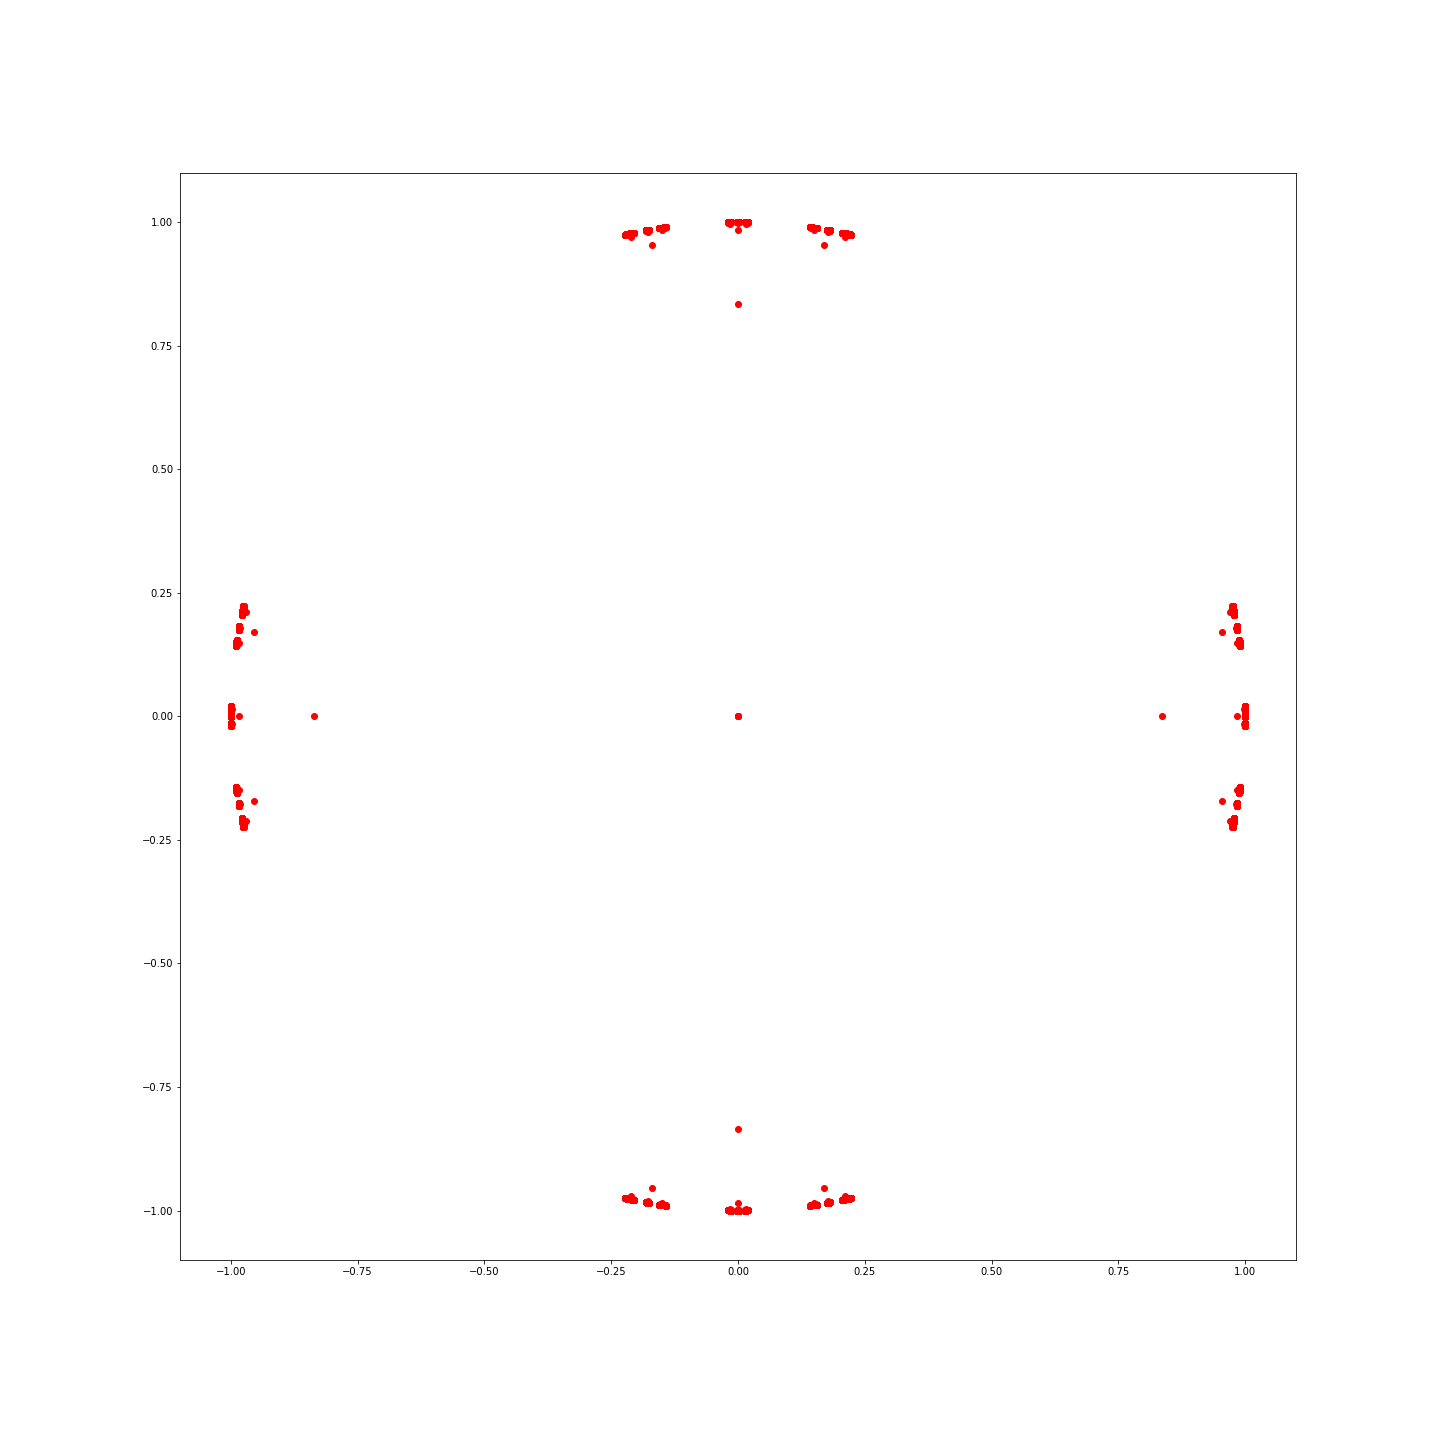
\includegraphics[width=0.386\textwidth]{Lambda=0.3,m=2,N=14.png}
\caption{$m=2$, $\Lambda=0.3$, $\theta\approx 33.398473447277695^{\circ}$, Level 14 ($N=14$).}
\end{figure}


\begin{figure}[H]
\centering
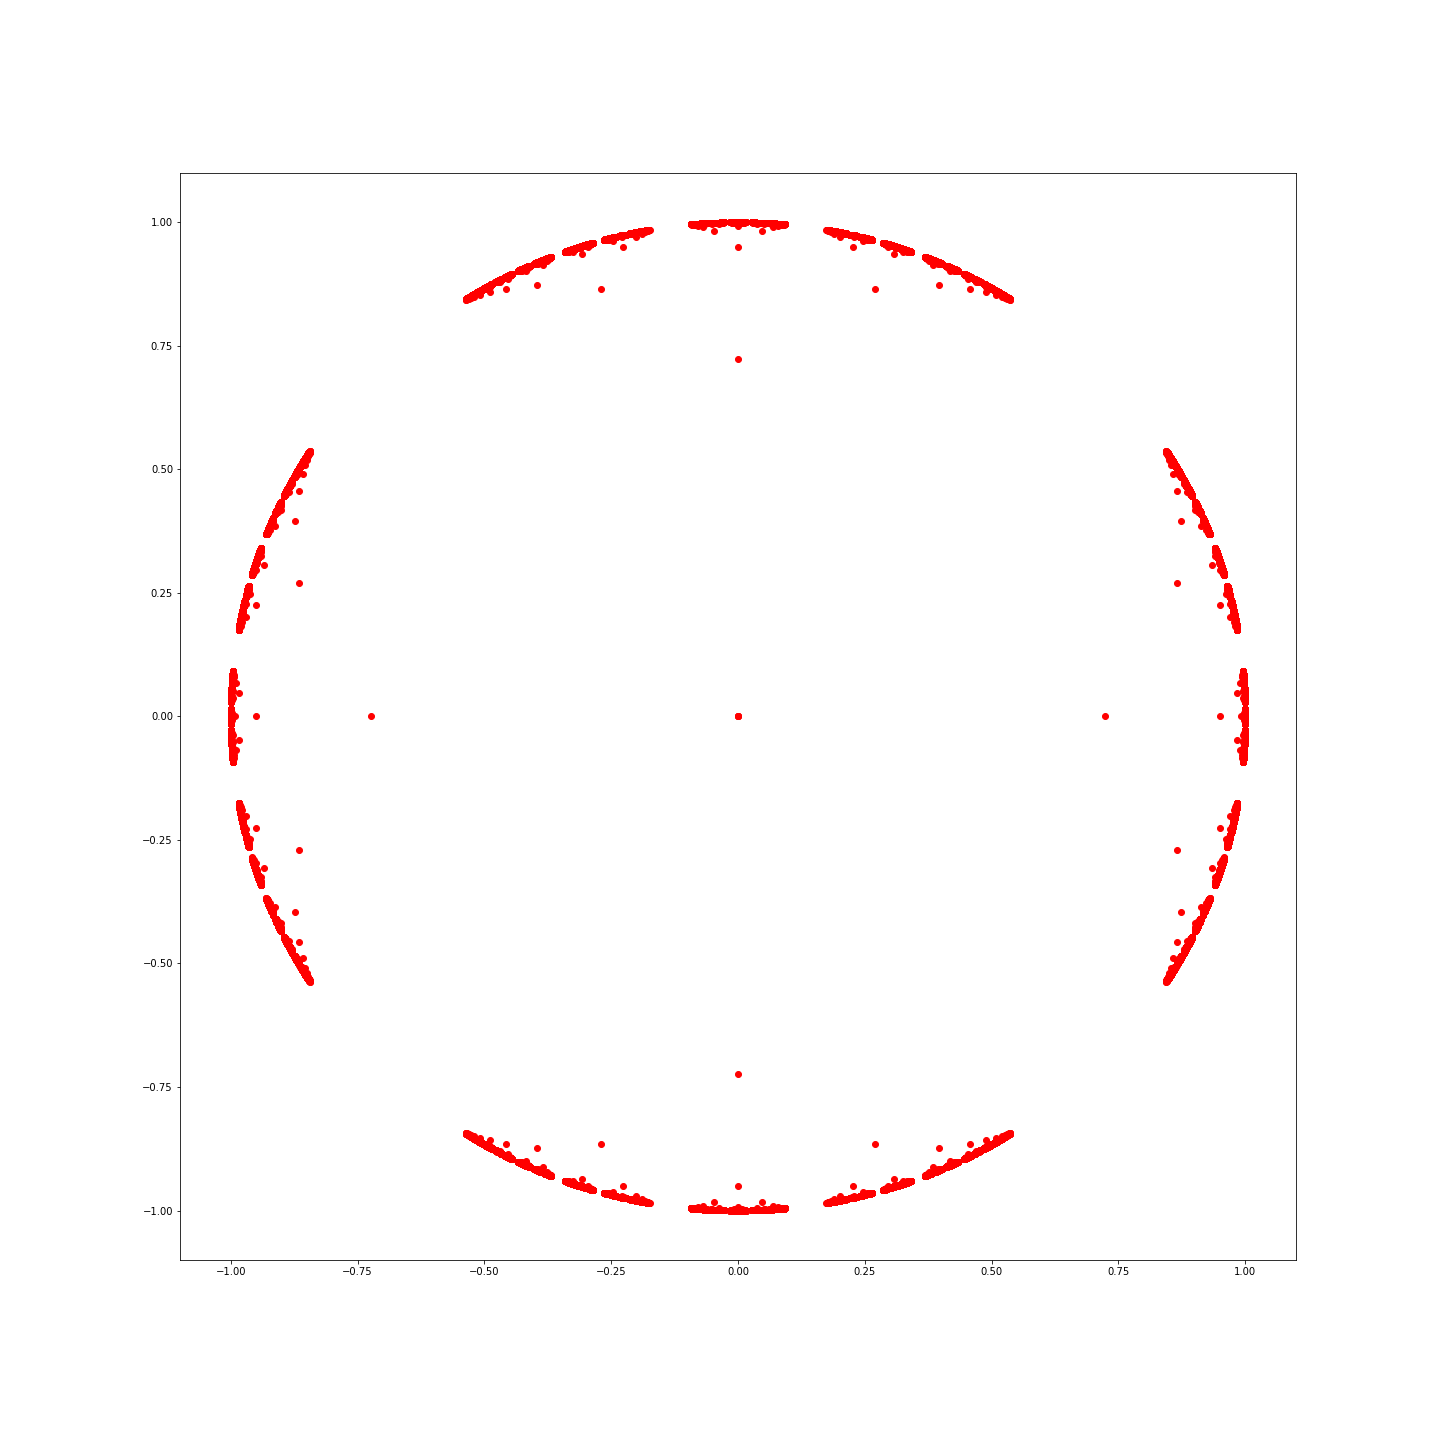
\includegraphics[width=0.386\textwidth]{Lambda=0.4,m=2,N=14.png}
\caption{$m=2$, $\Lambda=0.4$, $\theta\approx 43.602794482778144^{\circ}$, Level 14 ($N=14$).}
\end{figure}


\begin{figure}[H]
\centering
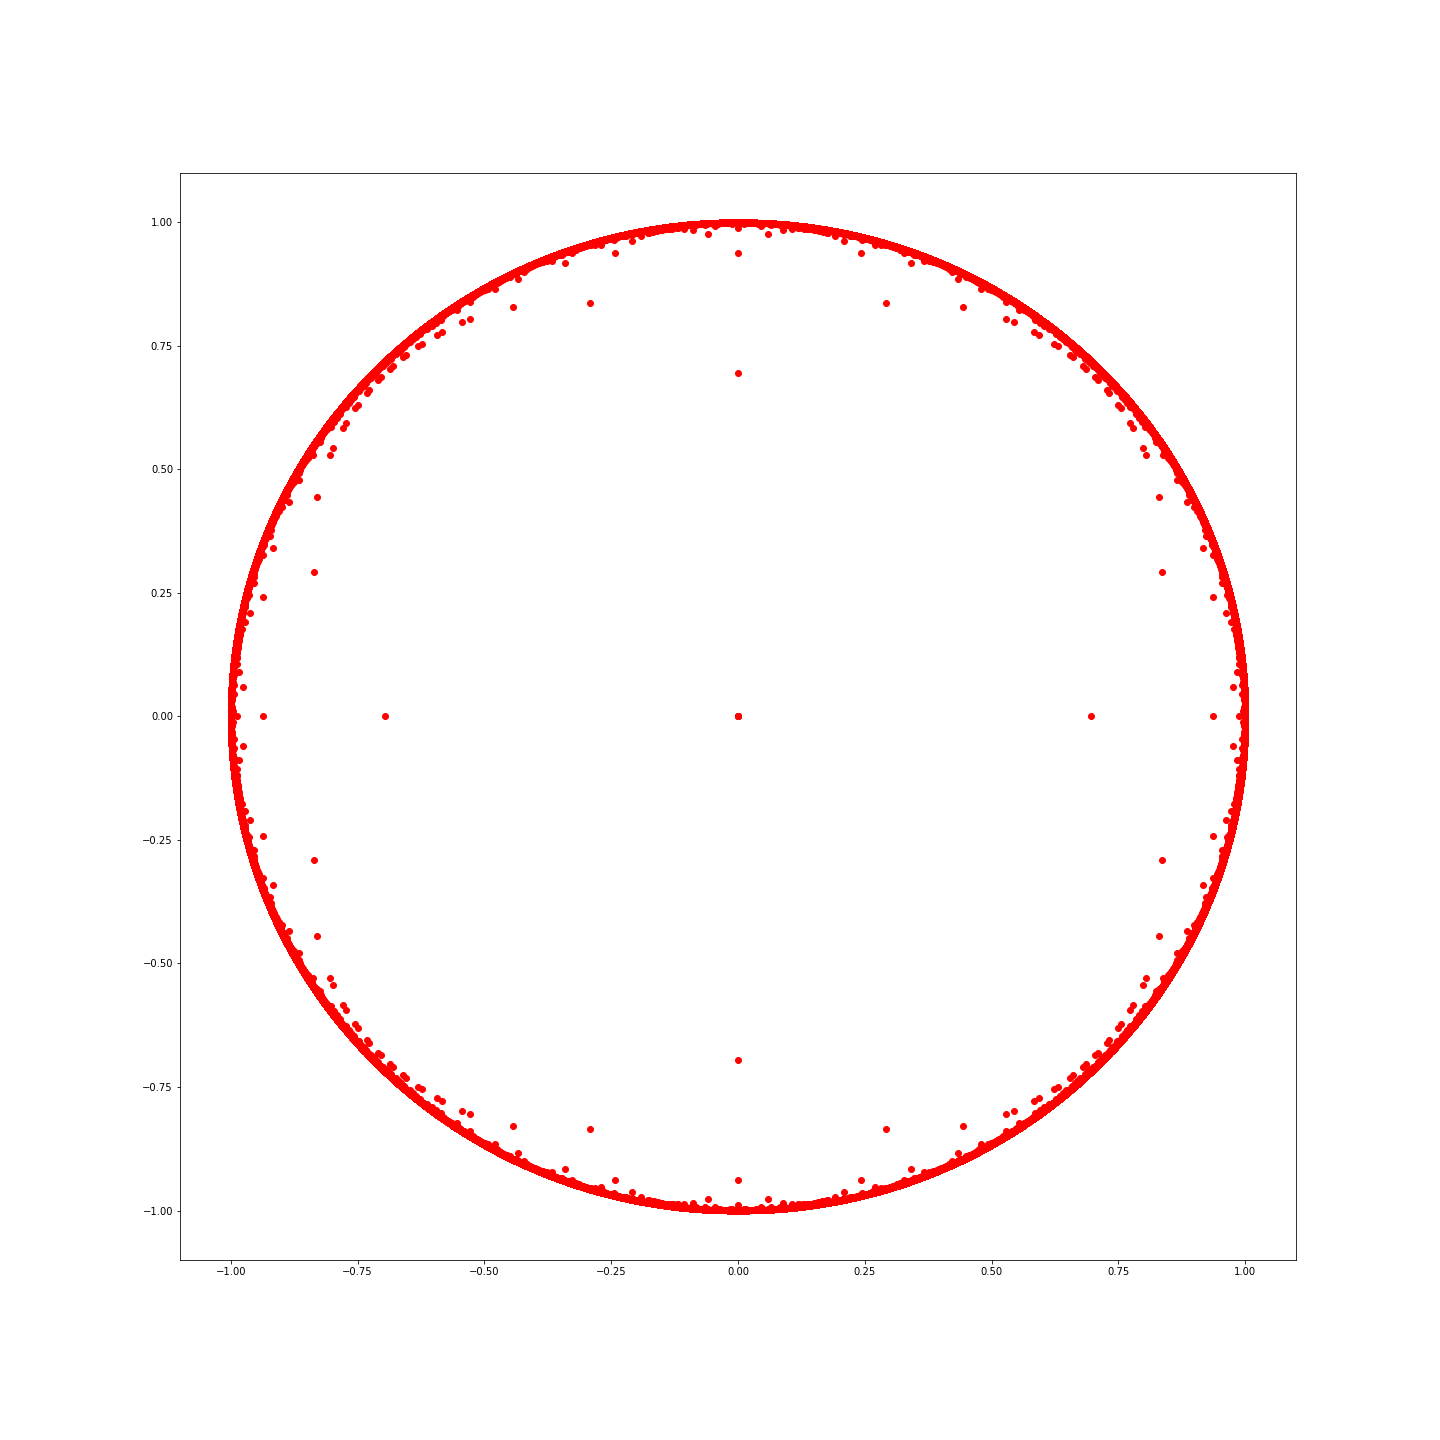
\includegraphics[width=0.386\textwidth]{Lambda=r+0.01,m=2,N=14.png}
\caption{{\scriptsize $m=2$, $\Lambda=\frac{\sqrt{2}}{2+\sqrt{2}}+0.01$, $\theta\approx 45.9746105715017^{\circ}$, Level 14 ($N=14$).}}
\end{figure}
\end{multicols}


\begin{multicols}{3}
\begin{figure}[H]
\centering
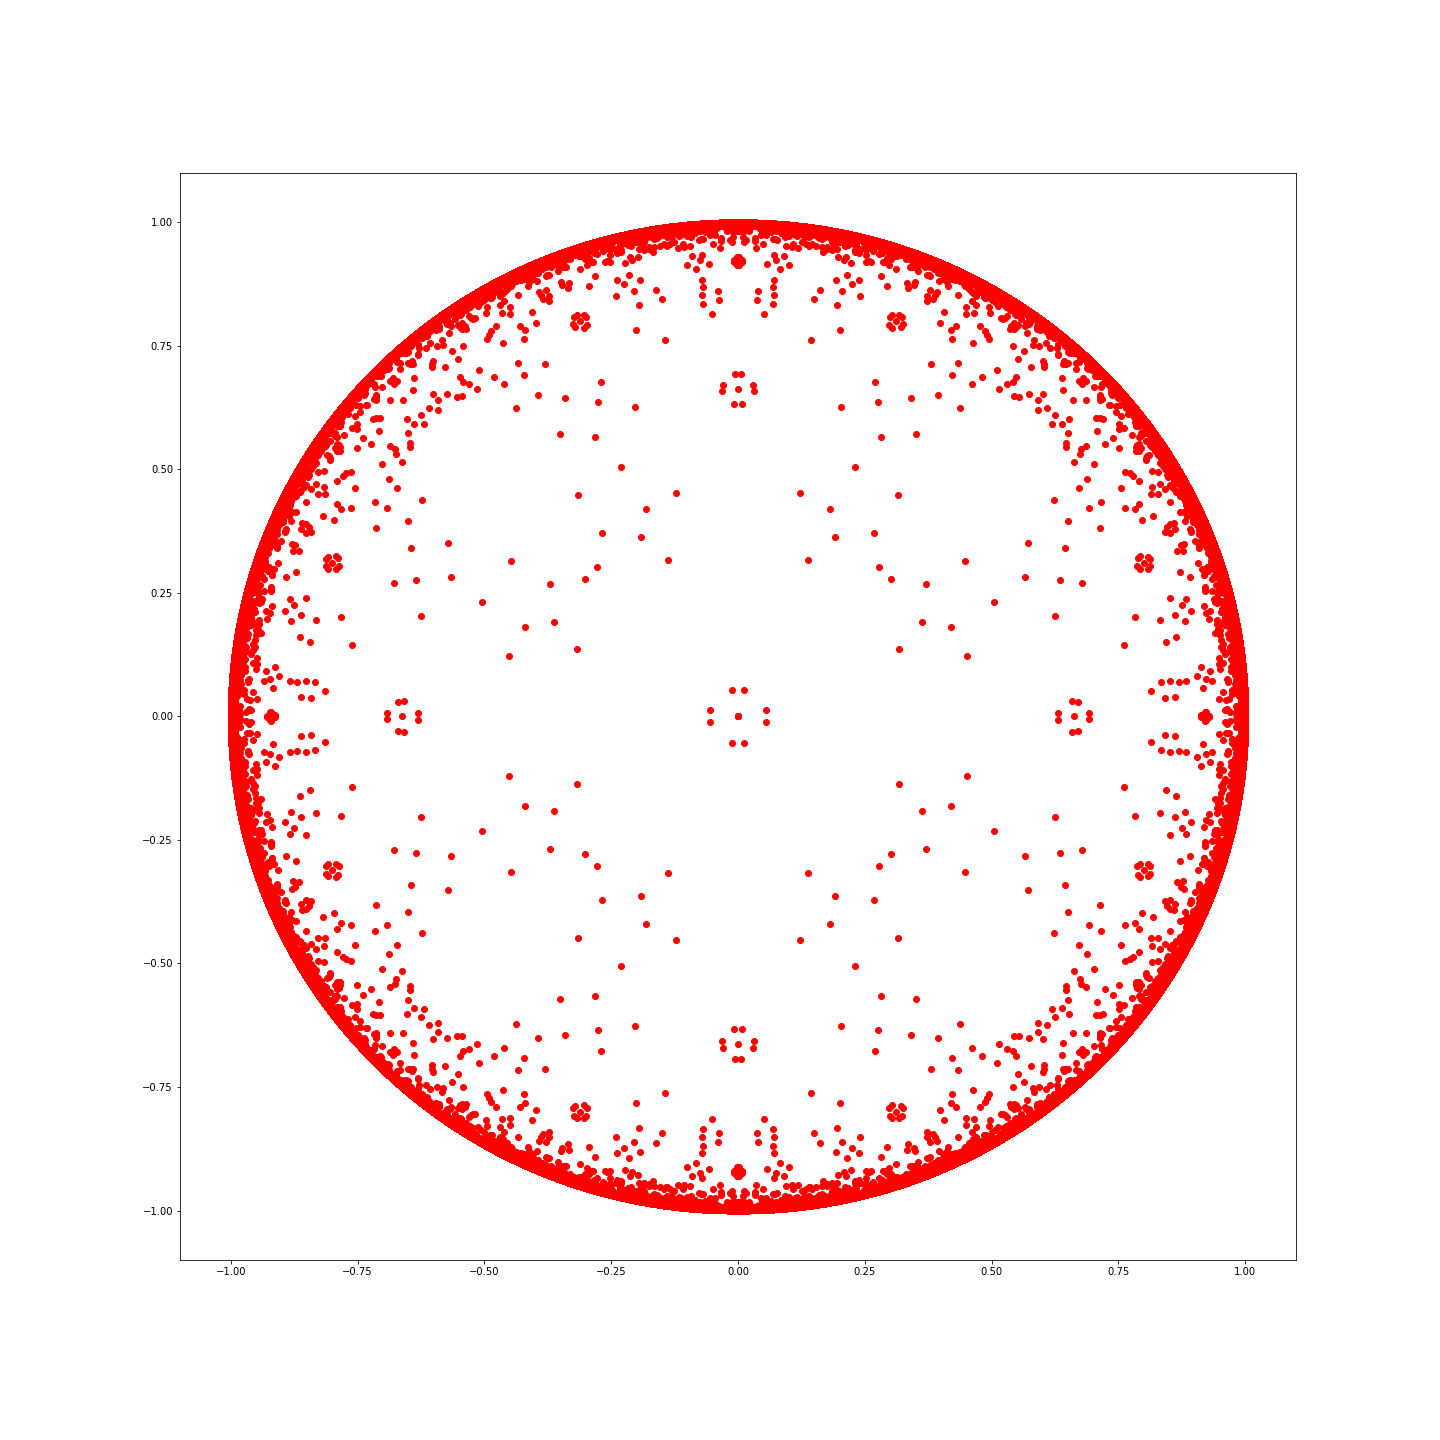
\includegraphics[width=0.386\textwidth]{Lambda=0.45,m=2,N=14.png}
\caption{{\scriptsize $m=2$, $\Lambda=0.45$, $\frac{\theta}{2}\approx 48.455517824418166^{\circ}$, Level 14 ($N=14$).}}
\end{figure}

\begin{figure}[H]
\centering
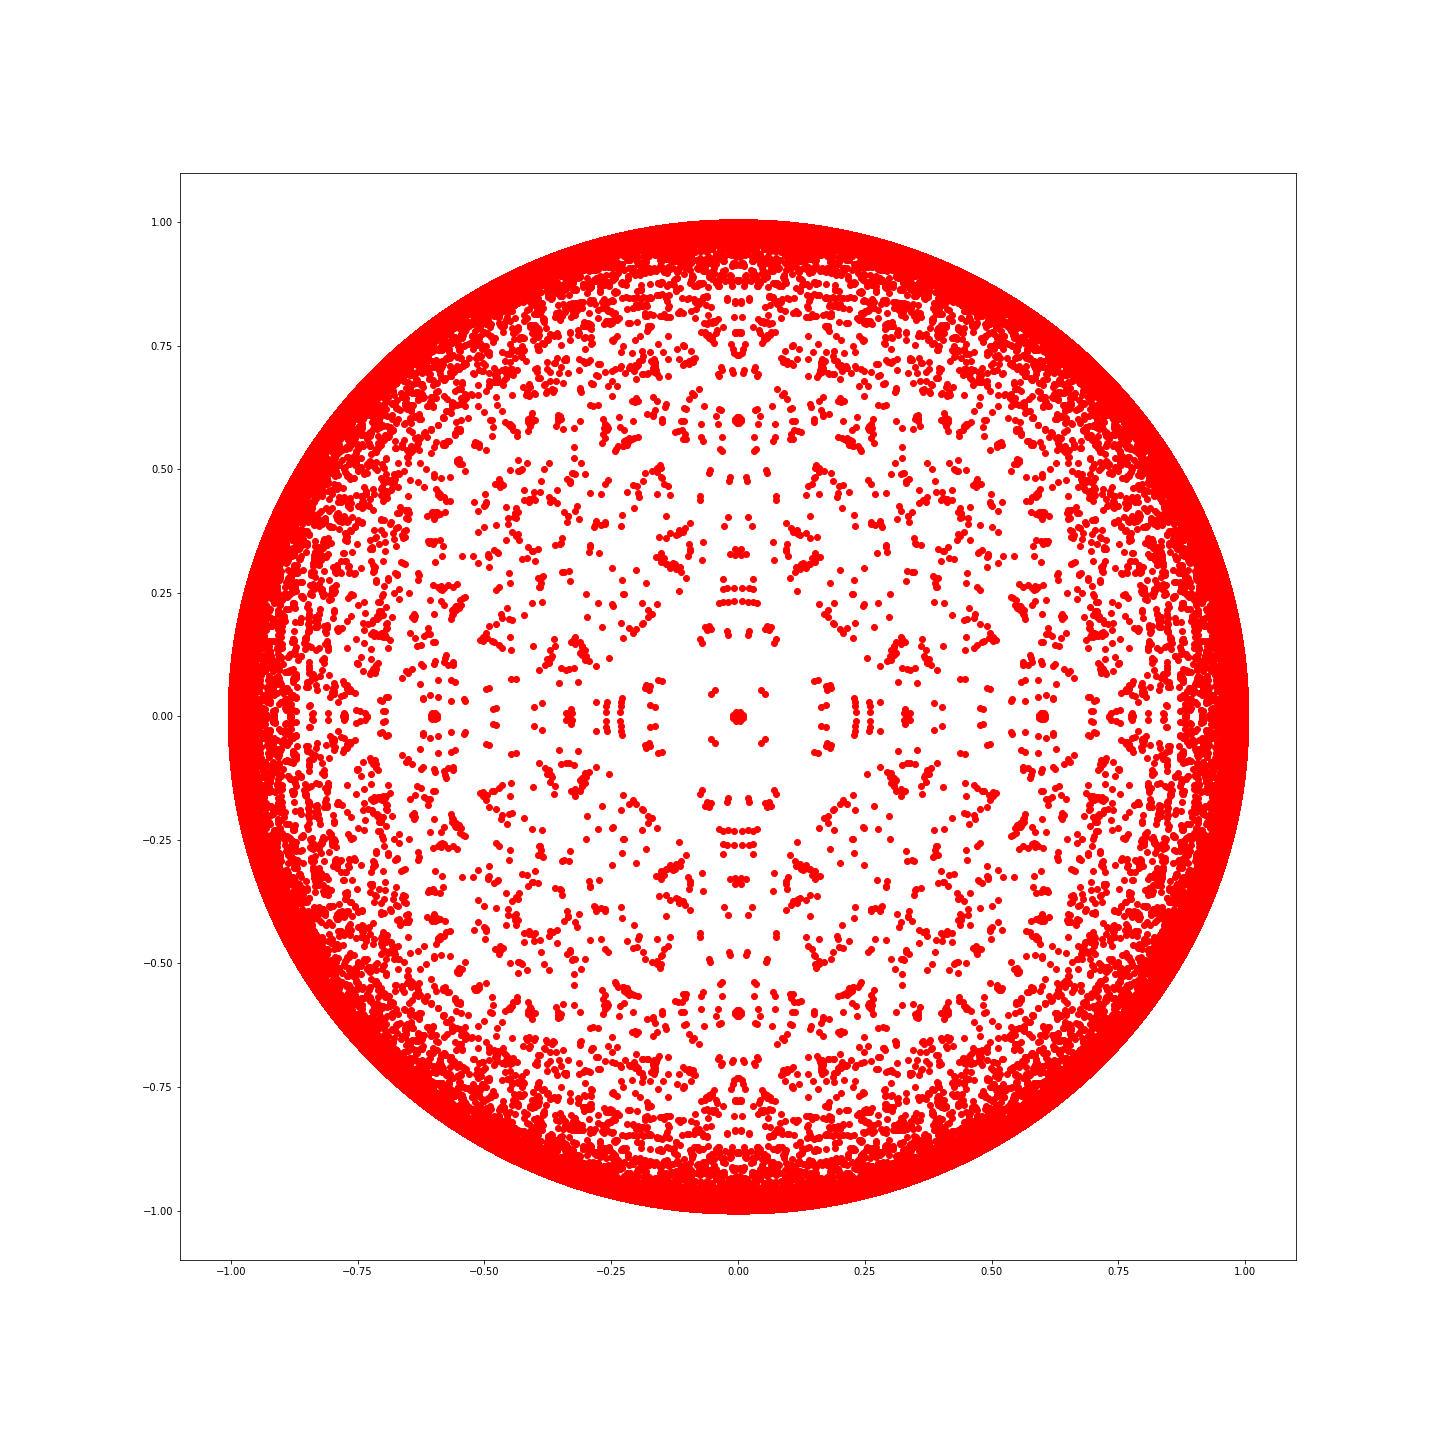
\includegraphics[width=0.386\textwidth]{Lambda=0.5,m=2,N=14.png}
\caption{{\scriptsize $m=2$, $\Lambda=0.5$, $\theta\approx 53.13010858755201^\circ$, Level 14 ($N=14$).}}
\end{figure}



\begin{figure}[H]
\centering
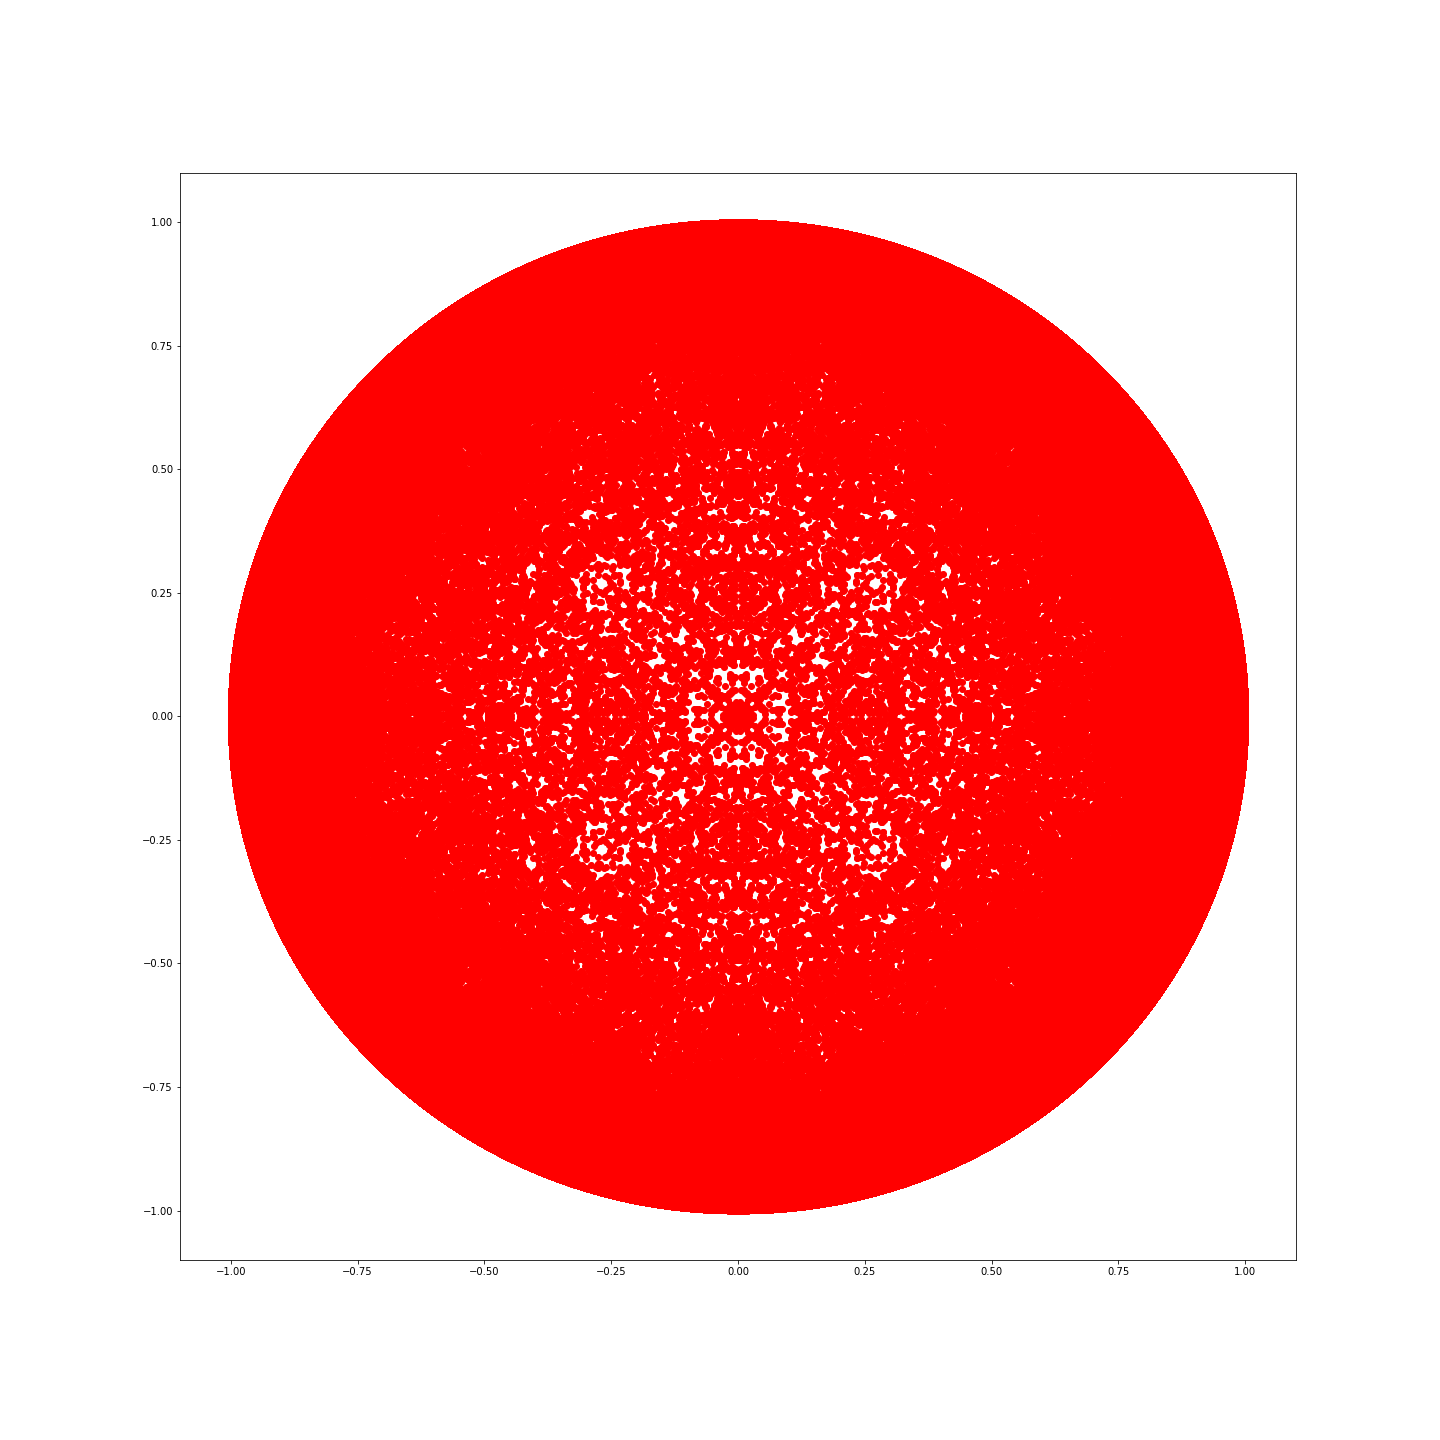
\includegraphics[width=0.386\textwidth]{Lambda=0.6,m=2,N=14.png}
\caption{{\scriptsize $m=2$, $\Lambda=0.6$, $\theta\approx 61.927531757108724^\circ$, Level 14 ($N=14$).}}
\end{figure}

\end{multicols}
\begin{scriptsize}
Our source code can be downloaded from GitHub: \newline
 \url{https://github.com/williamchuang/well-distributed-schottky-groups/tree/main/code}
\end{scriptsize}
\end{block}





\begin{alertblock}{Main Theorem}
\begin{footnotesize}
Suppose $\Gamma$ is a well-distributed Schottky group of order 2. Then, 
$$
\frac{\ln\left( 2+\frac{1}{1+2\sqrt{2}}\right)}{\ln\left(\cosh\left(r\right)\right)}\leq \delta\left(\Gamma\right)\leq
\min\left\lbrace \frac{\ln\left(4-\frac{2}{1+2\sqrt{2}}\right)}{\ln\left(\cosh\left(r\right)\right)},1\right\rbrace.
$$
\end{footnotesize}
\end{alertblock}
\begin{alertblock}{Conjecture}
\begin{footnotesize}
Suppose $\Gamma$ is a well-distributed Schottky group of order 2. Then, 
$$
\delta(\Gamma)=\frac{\ln\left( 3\right)}{\ln\left( \cosh\left( r\right)\right)},
$$
where
$
r=\ln\left(\frac{1+\vert T0\vert}{1-\vert T0 \vert} \right)=\ln\left(\frac{1+\cos\left(\frac{\theta}{2}\right)}{1-\cos\left(\frac{\theta}{2}\right)} \right),$ and $T0=\cos\left(\frac{\theta}{2}\right).$
\end{footnotesize}
\end{alertblock}




\begin{scriptsize}
Furthermore, the formula
$$
\bigg|\frac{\partial g_1}{\partial z}\bigg|=\frac{R^2}{\vert x_2-q_1\vert^2}
$$
can be used to check whether our conjecture can produce the same approximation based on McMullen's algorithm.

Furthermore, in general, by using cosine law, 
$$
\vert x_2-q_1\vert^2=2+\left(\tan^2\left(\frac{\theta}{2}\right)\right)+\sec\left(\frac{\theta}{2}\right),
$$
where $R=\tan\left(\frac{\theta}{2}\right)$. For $m=2$, by using cosine law for $\frac{\pi}{2}$, and solving $\alpha$ for $3(t)^\alpha=1$, we have the first level approximation as follows
$$
\delta(G)\approx \alpha=\frac{\ln\left(\frac{1}{3}\right)}{\ln\left(t \right)}
=\frac{\ln\left(\frac{1}{3}\right)}{\ln\left(\frac{\tan^2\left(\frac{\theta}{2}\right)}{2+\left(\tan^2\left(\frac{\theta}{2}\right)\right)} \right)}.
$$
\end{scriptsize}



\end{column}







\begin{column}{\sepwid}\end{column}% empty spacer column


\begin{column}{\onecolwid}



\begin{block}{Plotting $N=1$ theoretical, conjecture, and numerical results with bounds given by the main theorem}
\begin{figure}[H]
\centering
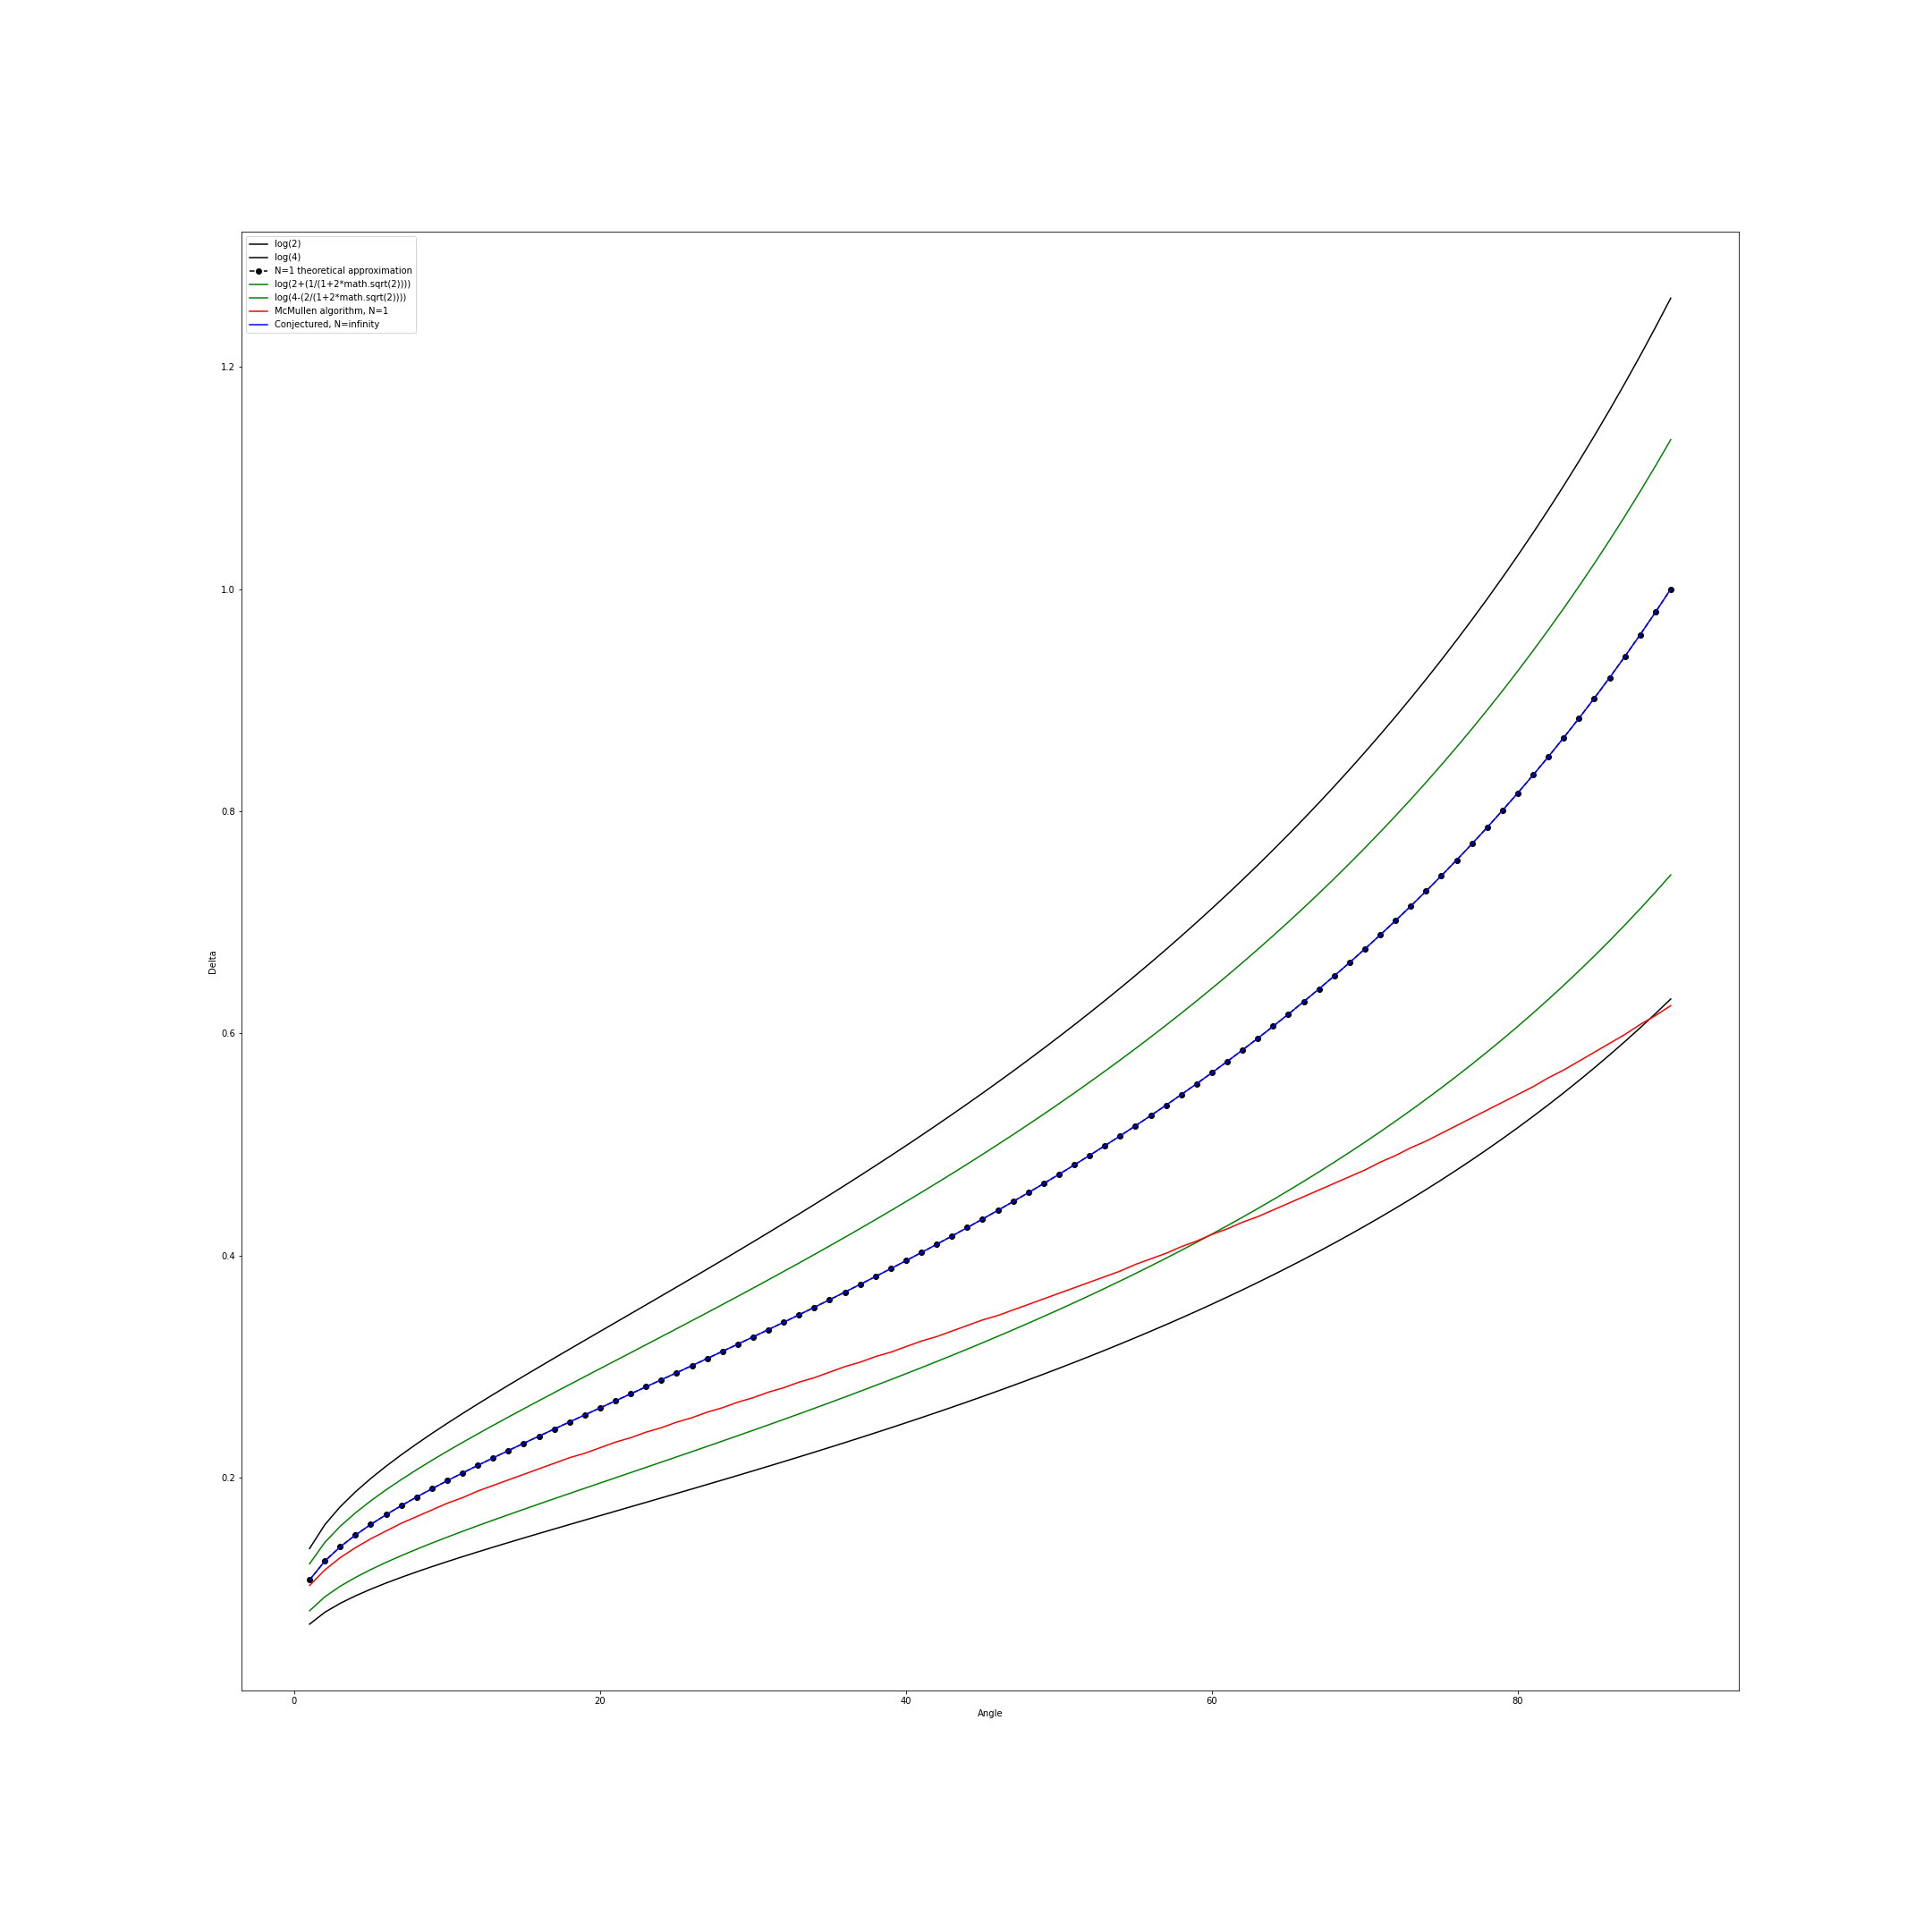
\includegraphics[width=0.8\textwidth]{Results from our main theorem, conjecture, and implementation of McMullen algorithm.png}
\caption{Results from our main theorems (colored in green and black), conjecture (blue), theoretical $N=1$ approximation (dotted black), and numerical $N=1$ approximation implementation of McMullen algorithm (red).}
\end{figure}
\end{block}



\begin{scriptsize}
Surprisingly, the findings of the $N=1$ approximation precisely match our conjecture for $N\to \infty$. Therefore, if our conjecture is true, then this implies that for a well-distributed Schottky group of rank $2$, $\delta(\Gamma)=\alpha_1(\Gamma)$. It may also imply that for all $N$, we have $$\delta(\Gamma)=\alpha_N(\Gamma)=\alpha_1(\Gamma)=\frac{\ln\left(\frac{1}{3}\right)}{\ln\left(\frac{\tan^2\left(\frac{\theta}{2}\right)}{2+\left(\tan^2\left(\frac{\theta}{2}\right)\right)} \right)}=\frac{\ln\left(3\right)}{\ln\left(\cosh\left(r\right)\right)}$$
 This alternate strategy might also shed some light on the meaning of $cosh(r)$ in our conjecture.

\end{scriptsize}



\begin{block}{Importance}
{\footnotesize Our main theorem gives sharp bounds on $\delta(\Gamma)$. Following the proof of the main theorem, for the first time, an exact form expression of Hausdorff dimension for two-generator Schottky group was conjectured and used to generate results against the best approximation derived using McMullen's algorithm.}
\end{block}

\begin{block}{Future Research}
{\footnotesize A proof of the conjecture, a generalization to $m>2$, and enhancements to our implementations are on the horizon for our future work. Due to there are heavily matrix operations involved, an implementation on parallel computing in a contemporary computer might potentially enhance McMullen's results.}
\end{block}

\begin{block}{References}
\bibliographystyle{amsplain}
\addcontentsline{toc}{chapter}{Bibliography}

{\tiny \bibliography{thesis}}
%\rmfamily{\begin{enumerate}
%\item N. Alon and M. Tarsi, A Note on Graph Colorings and Graph Polynomials, Journal of Combinatorial Theory, Series B 70, 197-201 (1997).

%\item O. Ore, "The Four Color Problem,'' pp. 180-185,  Academic Press, New York, 1967.

%\item T. Zaslavsky. Signed Graph Coloring. Discrete Mathematics, 39(2):215-228, 1982.

%\end{enumerate}}
\end{block}
\end{column}%This is the end of the "sub-poster."  (Remember, the subposter is a column that's \twocolwid wide.)
\end{columns}%This is the end of the big "columns" environment for the whole poster.
\end{frame}
\end{document}
